\chapter{Deus et Eliseus venerunt in mundum}
\begin{center}
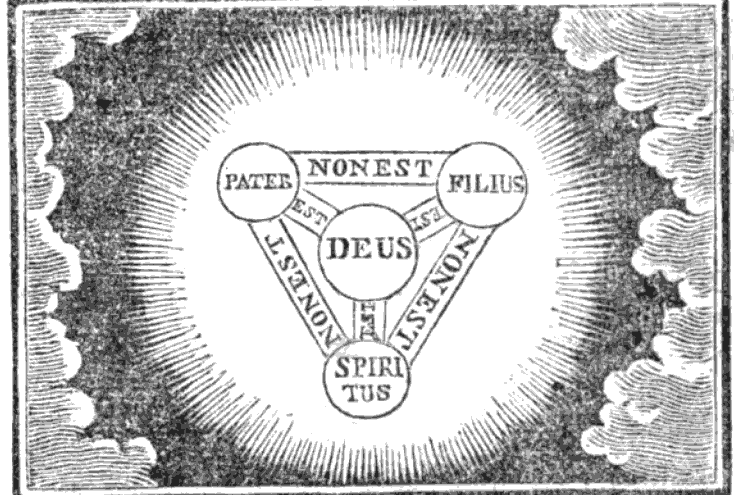
\includegraphics[scale=1.5]{God.png}
\end{center}

\section{Intended Audience}
This is intended for students who have completed Lectio 2 of Latin by the Natural Method and Chapter 3 of Lingua Latina Per Se Illustrata.

\section{Text}
Deus tenuit Eliseum et ostendit Eliseo mundum. Mundus est rotundus. Etiam Deus ostendit Eliseo Caelum. Caelum habet stellas. Stellae habent ignem in semetipis.  Moyses scripsit in Geneseo, Deus fecit in caelo luminaria. Maius luminarium regnat diem, et minora luminaria regnat noctem. Maius Eliseus fuit propheta. Minus Eliseus est filius meus parvus. In nocte sunt stellae et luna. Stellae et Luna splendent in nocte. Luna maius luminarium in nocte. Stellae minores sunt luminaria in nocte. 